\documentclass[11pt, letterpaper]{article}

\usepackage[utf8]{inputenc}
\usepackage[T1]{fontenc}
\usepackage{lmodern}
\usepackage{graphicx}
\usepackage{longtable}
\usepackage{wrapfig}
\usepackage{rotating}
\usepackage{amsmath}
\usepackage{textcomp}
\usepackage{amssymb}
\usepackage{hyperref}
\usepackage[spanish]{babel}
\usepackage[round]{natbib}
\usepackage{subcaption}

\title{\bfseries Tarea}
\author{Ángel García Báez}
\date{\today}
\setcounter{tocdepth}{4} 

\begin{document}
	
	% Página de presentación
	\begin{titlepage}
		\centering
		
\includegraphics[width=0.2\textwidth]{logo.png}\par
		\vspace{1cm}
		{\LARGE \bfseries Universidad Veracruzana \par}
		\vspace{1cm}
		{\Large Maestría en Inteligencia Artificial\par}
		\vspace{3cm}
		{\LARGE \bfseries Lógica difusa \par}
		\vspace{1cm}
		{\Large \bfseries Tarea 2. Problema del mesero y problema del confort con lógica difusa programado paso a paso en MATLAB. \par}
		\vfill
		{\Large \textit{Ángel García Báez}\par}
		\vfill
		{\Large Dr. Sergio Hernández Méndez \par}
		\vfill
		{\Large \today \par}
	\end{titlepage}
	
	% Página exclusiva para la tabla de contenidos
	\newpage
	\tableofcontents
	\newpage
	
	% Sección para el problema 1
	
	\section{Introducción}
	
	
	\newpage
	
	
	
	\section{Problema 1: Problema del mesero}
	
	\subsection{Explicación del Problema}
	
	Se tiene el problema de determinar cuanta propina dejarle a un mesero en un restaurante después de comer. Para ello, se toman en cuenta las variables de Servicio y la Comida.
	
	\subsection{Variables y sus codificaciones}
	
	
	A continuación se listan los valores de las variables lingüísticas que se propusieron para SERVICIO, COMIDA y PROPINA como sigue:
	
	
	\begin{enumerate}
		\item Servicio: Malo (0,4), Regular (3.5,8) y Bueno (7.5,10).
		\begin{figure}[h]
			\centering
			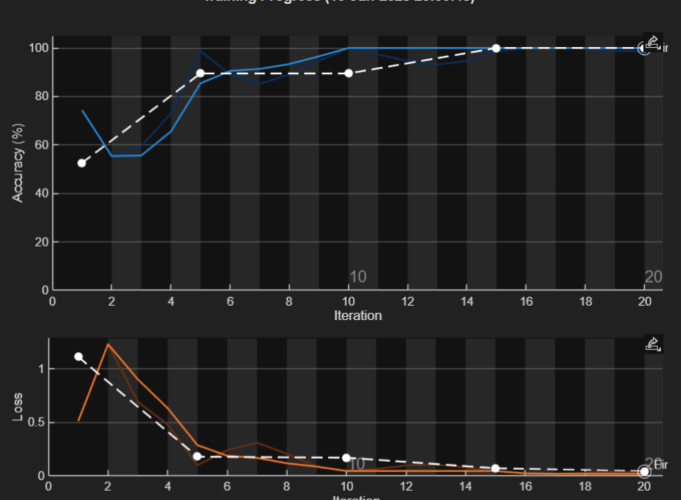
\includegraphics[width=0.8\textwidth]{IMG/G1.png}
		\end{figure}
		
		\item Comida: Malo (0,30), Normal (25,60), Buena (50,95) y Excelente (85 a 100).
		\begin{figure}[h]
			\centering
			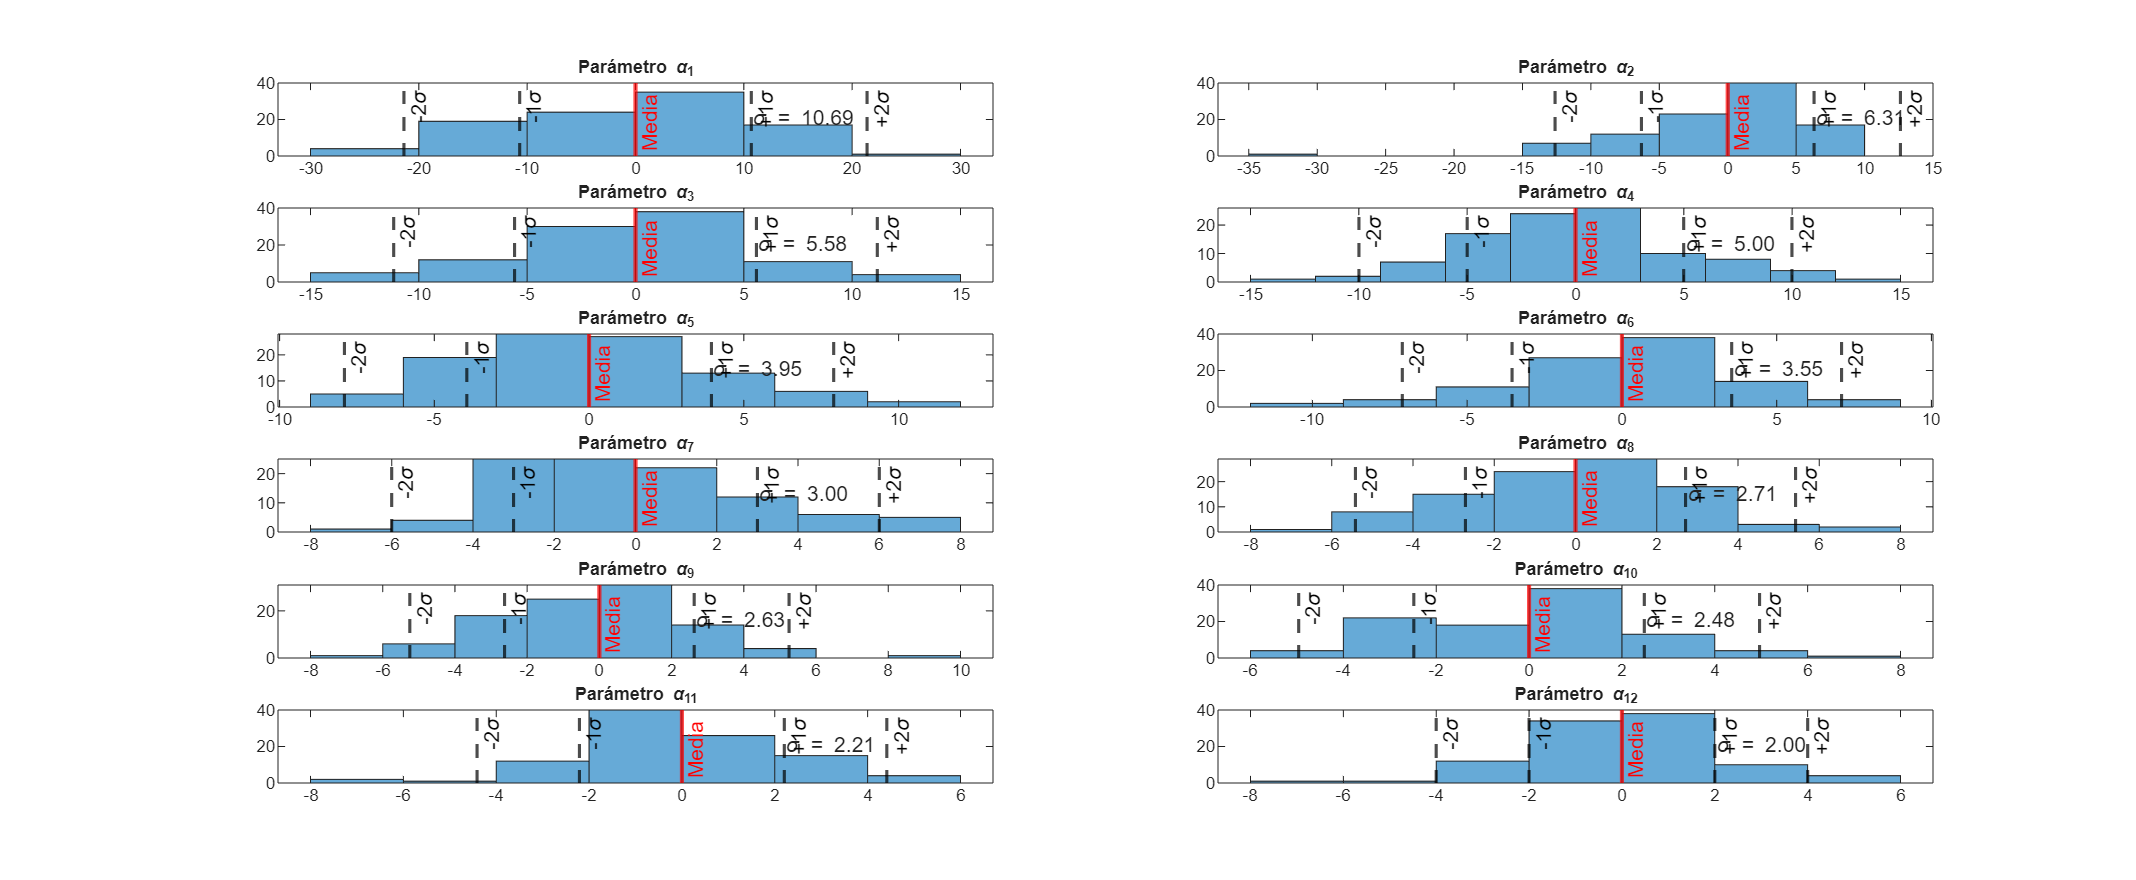
\includegraphics[width=0.8\textwidth]{IMG/G2.png}
		\end{figure}
		\newpage
		\item Propina: Baja (0 a 5), Normal (4 a 14.5) y Alta (11,20).
		\begin{figure}[h]
			\centering
			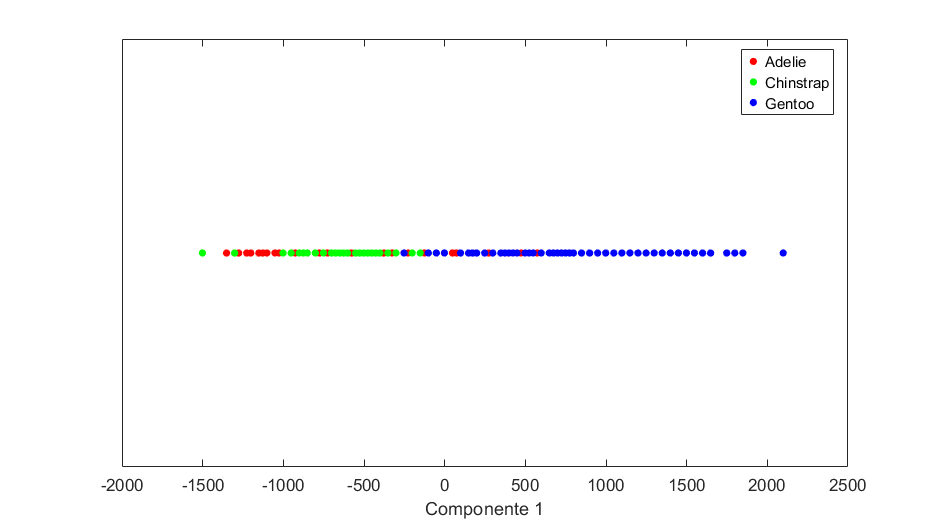
\includegraphics[width=0.8\textwidth]{IMG/G3.png}
		\end{figure}
	\end{enumerate}
	
	Cabe mencionar que todas las funciones de membresía se están modelando haciendo uso de la función trapezoidal y con el método de defuzzificación de centroide. \\
	
	Posterior a la propuesta de los rangos de calificación para la comida y el servicio, así como la determinación del porcentaje de propina que va de 0 a 20\%, se procede con el diseño de la base del conocimiento para que sea posible realizar las inferencias para el porcentaje de propina.
	
	\subsection{Reglas de inferencia.}
	
	A continuación se muestran las doce reglas que se construyeron para este problema:
	
	\begin{enumerate}
		\item R1: Si \textbf{SERVICIO} es \textbf{\textit{MALO}} y la \textbf{COMIDA} es \textbf{\textit{MALA}}, la \textbf{PROPINA} es \textbf{\textit{BAJA}}.
		\item R2: Si \textbf{SERVICIO} es \textbf{\textit{BUENO}} y la \textbf{COMIDA} es \textbf{\textit{NORMAL}}, la \textbf{PROPINA} es \textbf{\textit{NORMAL}}.
		\item R3: Si \textbf{SERVICIO} es \textbf{\textit{REGULAR}} y la \textbf{COMIDA} es \textbf{\textit{NORMAL}}, la \textbf{PROPINA} es \textbf{\textit{NORMAL}}.
		\item R4: Si \textbf{SERVICIO} es \textbf{\textit{REGULAR}} y la \textbf{COMIDA} es \textbf{\textit{BUENA}}, la \textbf{PROPINA} es \textbf{\textit{NORMAL}}.
		\item R5: Si \textbf{SERVICIO} es \textbf{\textit{BUENO}} y la \textbf{COMIDA} es \textbf{\textit{EXCELENTE}}, la \textbf{PROPINA} es \textbf{\textit{ALTA}}.
		\item R6: Si \textbf{SERVICIO} es \textbf{\textit{MALO}} y la \textbf{COMIDA} es \textbf{\textit{EXCELENTE}}, la \textbf{PROPINA} es \textbf{\textit{BAJA}}.
		\item R7: Si \textbf{SERVICIO} es \textbf{\textit{BUENO}} y la \textbf{COMIDA} es \textbf{\textit{MALA}}, la \textbf{PROPINA} es \textbf{\textit{BAJA}}.
		\item R8: Si \textbf{SERVICIO} es \textbf{\textit{MALO}} y la \textbf{COMIDA} es \textbf{\textit{NORMAL}}, la \textbf{PROPINA} es \textbf{\textit{BAJA}}.
		\item R9: Si \textbf{SERVICIO} es \textbf{\textit{MALO}} y la \textbf{COMIDA} es \textbf{\textit{BUENA}}, la \textbf{PROPINA} es \textbf{\textit{BAJA}}.
		\item R10: Si \textbf{SERVICIO} es \textbf{\textit{BUENO}} y la \textbf{COMIDA} es \textbf{\textit{BUENA}}, la \textbf{PROPINA} es \textbf{\textit{ALTA}}.
		\item R11: Si \textbf{SERVICIO} es \textbf{\textit{REGULAR}} y la \textbf{COMIDA} es \textbf{\textit{MALA}}, la \textbf{PROPINA} es \textbf{\textit{BAJA}}.
		\item R12: Si \textbf{SERVICIO} es \textbf{\textit{REGULAR}} y la \textbf{COMIDA} es \textbf{\textit{EXCELENTE}}, la \textbf{PROPINA} es \textbf{\textit{ALTA}}.
	\end{enumerate}
	
	
	\subsection{Gráficos}
	
	La gráfica de superficie resultante de todo lo descrito previamente, es la siguiente:
	
	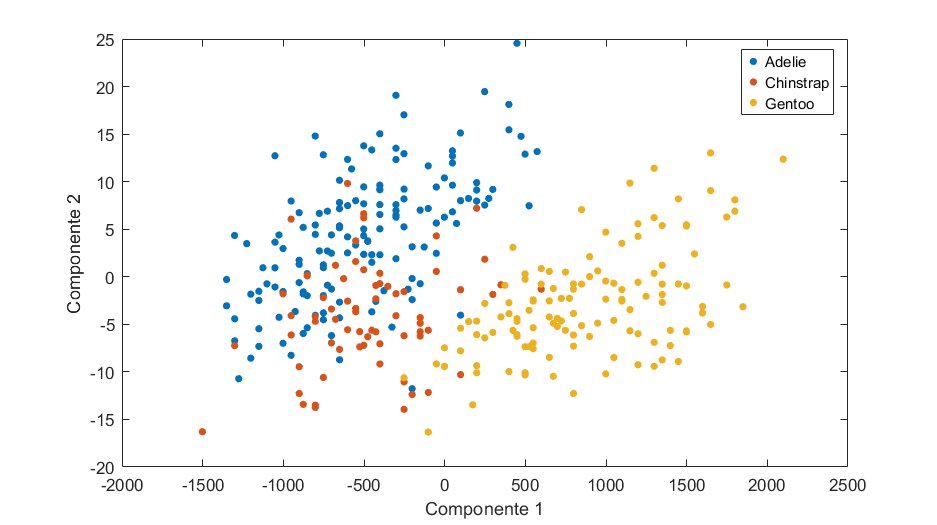
\includegraphics[width=0.8\textwidth]{IMG/G4.png}
	
	La superficie formada presenta cambios muy abruptos, junto con zonas de estancamiento y dista mucho de presentar un comportamiento "suave".
	
	\newpage
	
	Complementariamente, se observa en el gráfico de las reglas de inferencia que no parecen activar un rango más amplio de las mismas, lo que se traduce en lo que se observa dentro de la gráfica de superficie, hay zonas donde por más que se combinen las reglas, no hay forma de cambiar el resultado. \\
	
	
	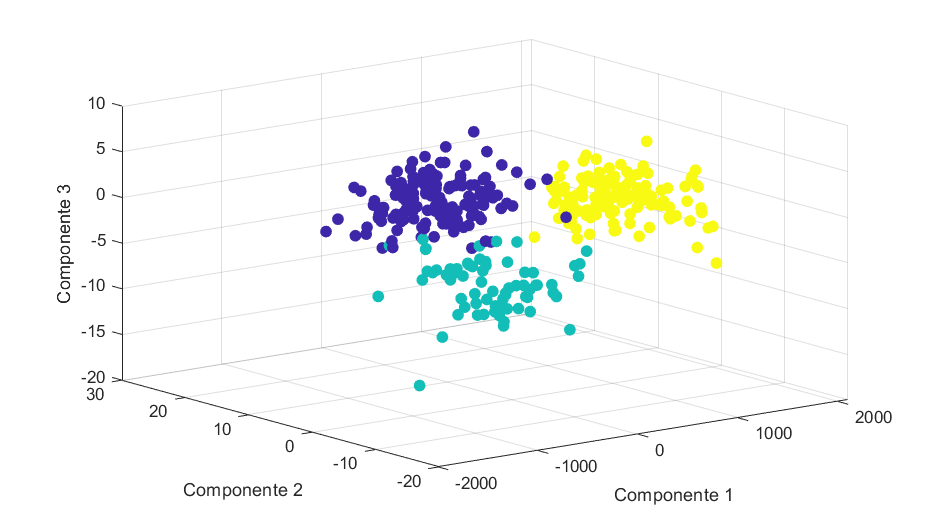
\includegraphics[width=1.1\textwidth]{IMG/G5.png}
	
	
	
	
	\newpage
	
	\subsection{Propuestas de mejora}
	\subsubsection{Propuesta 1: Añadir todas las posibles reglas}
	
	Como primer propuesta de mejorar el modelado del problema, se propone aumentar la base de reglas para que tome en cuenta las 36 posibles combinaciones de reglas que se pueden formar. Para ello, solo se modificaron las reglas, se mantuvieron los rangos, las funciones de membresía trapezoidales y la desfuzzificación con el método del centroide.
	
	A continuación se muestra el resultado de las gráficas de superficie junto con las de función de activación: \\
	
	
	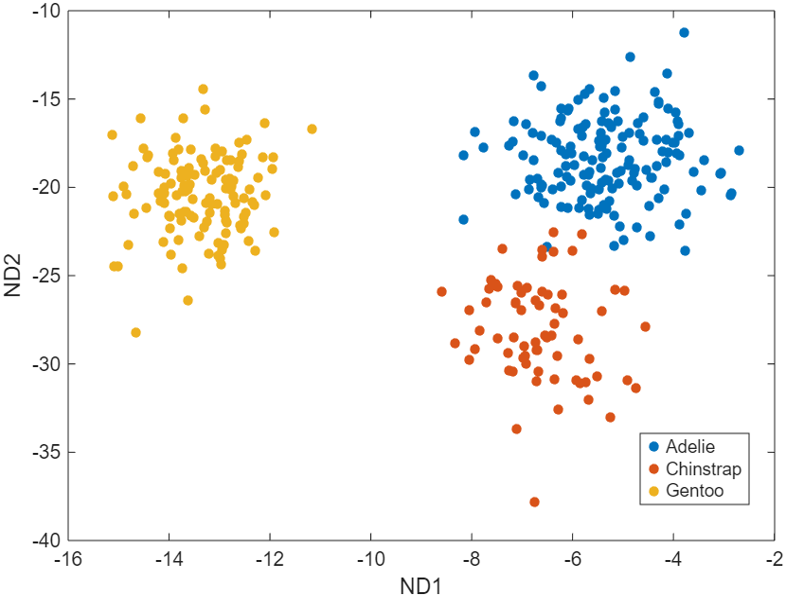
\includegraphics[width=1.1\textwidth]{IMG/G6.png} \\
	
	La gráfica de superficie dista mucho de acercarse a un comportamiento suave, al contrario, al haber reglas idénticas pero que conducen a 3 resultados distintos, tal parece que segmento la gráfica en esos 3 posibles escenarios.
	
	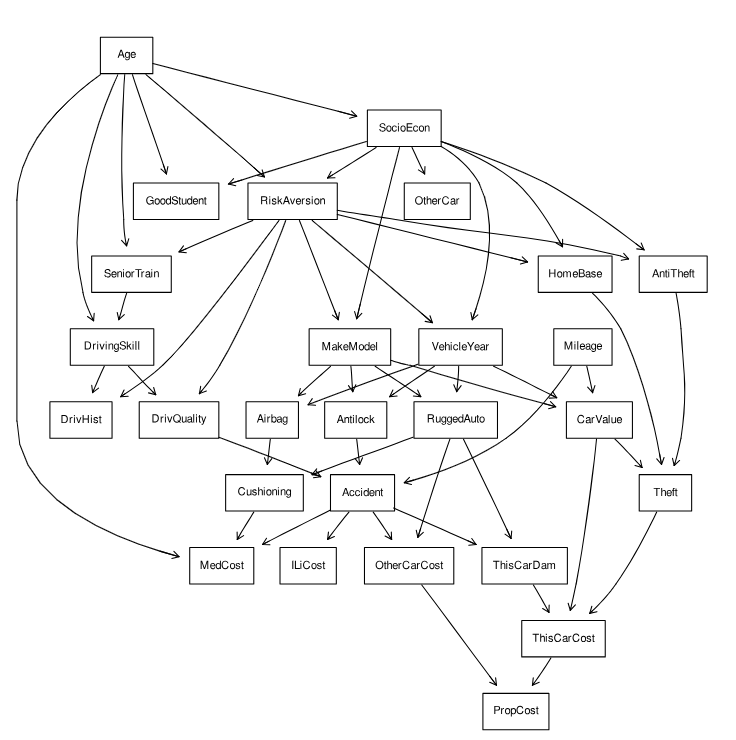
\includegraphics[width=1.1\textwidth]{IMG/G7.png} \\
	
	La gráfica de las reglas, muestra la activación de varias reglas, pero al estar variando los valores del SERVICIO y la COMIDA, la PROPINA no presentaba cambios en sus valores.
	
	
	\newpage
	
	\subsubsection{Propuesta 2: Regresar a la base con las 12 reglas originales y aplicar funciones de membresía singleton}
	
	Dado que no se observan cambios favorables con la implementación de todas las reglas, se decidió volver a la base de las 12 reglas originales pero, haciendo modificaciones a las funciones de membresía, tomando funciones triangulares y fijándolas en un valor para que la tome como una función singleton.
	
	Se aplicaron los cambios de funciones de membresía para la variable PROPINA como se especifica a continuación
	
	\begin{enumerate}
		\item Propina: Baja (3), Normal (10) y Alta (15).
		\begin{figure}[h]
			\centering
			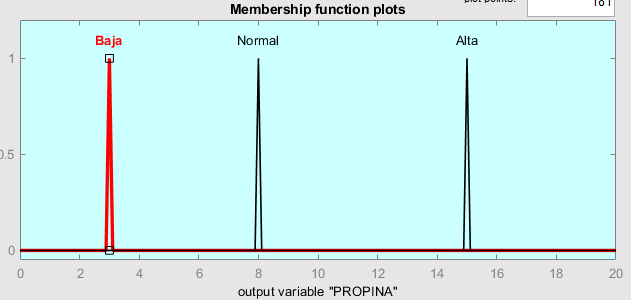
\includegraphics[width=0.8\textwidth]{IMG/G9.png}
		\end{figure}
	\end{enumerate}
	
	
	\newpage 
	
	La gráfica de superficie asociada a este cambio se muestra a continuación. \\
	
	
	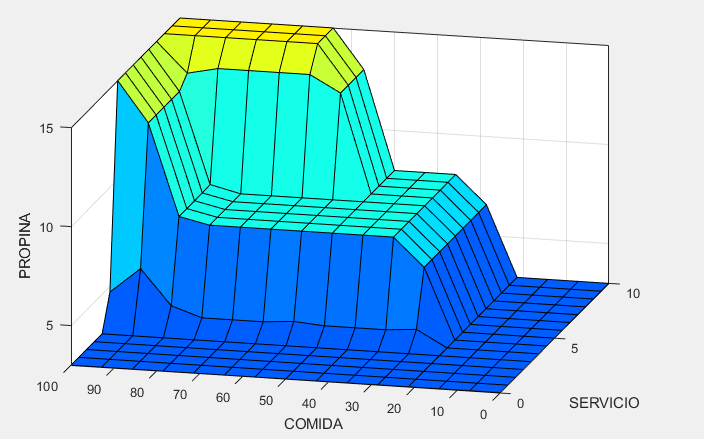
\includegraphics[width=0.8\textwidth]{IMG/G8.png} \\
	
	Se observa como este cambio de funciones de membresía a singleton en la variable PROPINA, no tuvo un impacto significativo en la gráfica respecto al caso base del problema. \\
	
	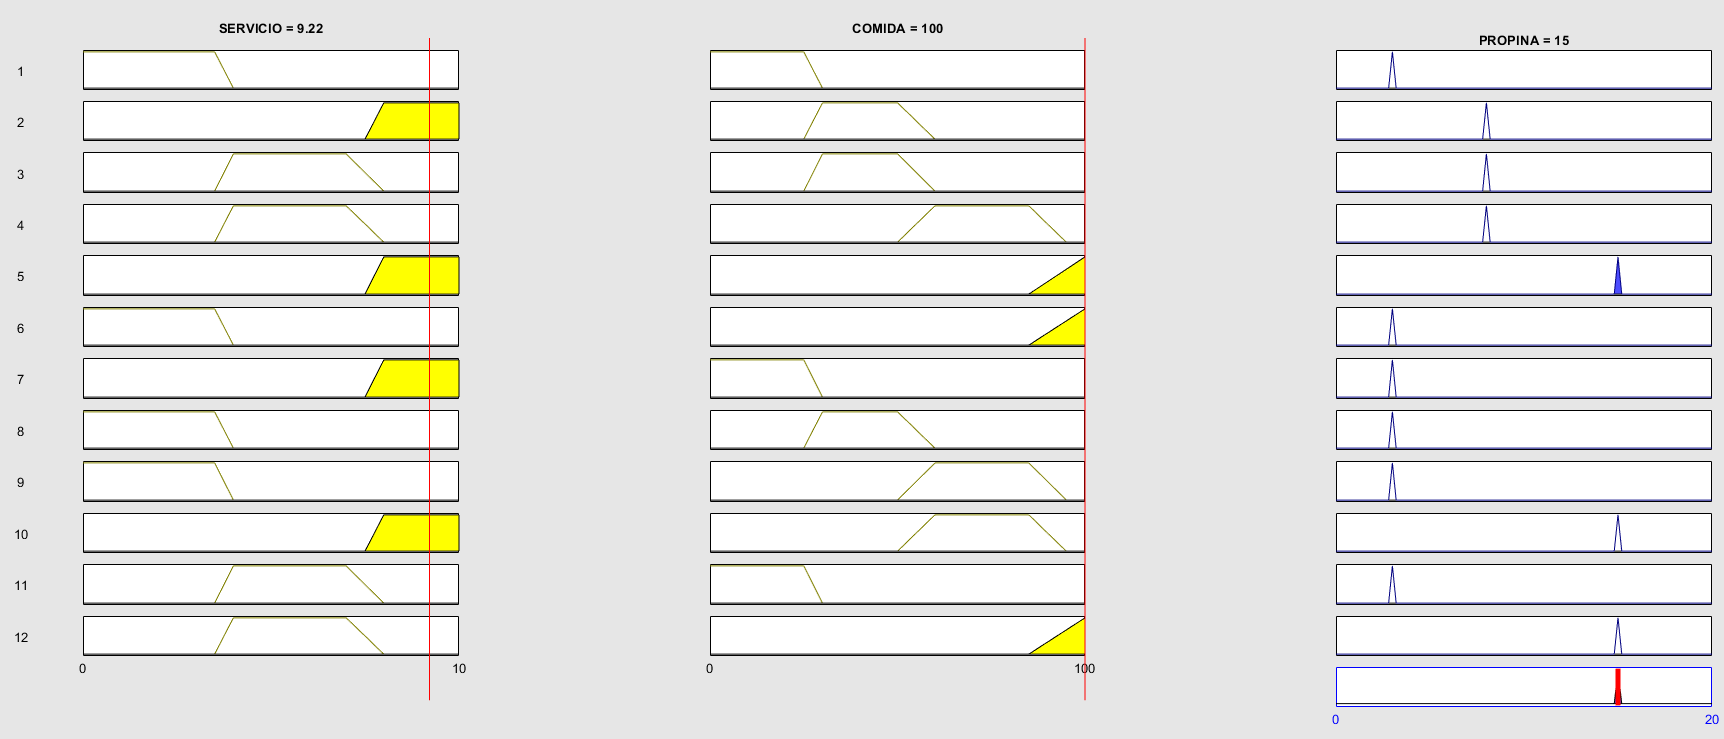
\includegraphics[width=1\textwidth]{IMG/G10.png}
	
	La gráfica de reglas muestra como se activan las funciones singleton en puntos muy específicos. \\
	
	
	
	\newpage
	
	\subsubsection{Propuesta 3: Regresar a la base con las 12 reglas originales y aplicar funciones de membresía GAUSSIANAS}
	
	Con la finalidad de lograr suavizar la gráfica de superficie, se propone implementar cambios en los rangos de los valores de cada una de las variables lingüísticas y modificar sus funciones de membresía con gaussianas sin tocar las reglas ya construidas previamente.
	
	A continuación se listan los valores de las variables lingüísticas que se propusieron para SERVICIO, COMIDA y PROPINA como sigue:
	
	
	\begin{enumerate}
		\item Servicio: Malo ($\mu = 1.5$, $\sigma = 2$), Regular ($\mu = 5$, $\sigma = 1.5$) y Bueno ($\mu = 7.5$, $\sigma = 1.5$).
		\begin{figure}[h]
			\centering
			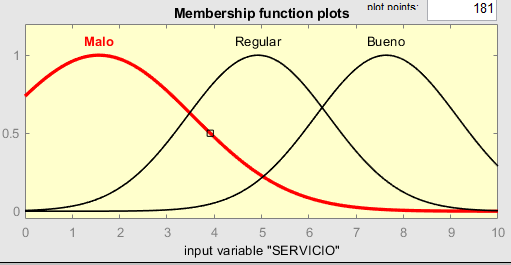
\includegraphics[width=0.8\textwidth]{IMG/G14.png}
		\end{figure}
		
		\item Comida: Malo ($\mu = 15$, $\sigma = 15$), Normal ($\mu = 45.5$, $\sigma = 15$), Buena ($\mu = 66$, $\sigma = 10$) y Excelente ($\mu = 90$, $\sigma = 15$).
		\begin{figure}[h]
			\centering
			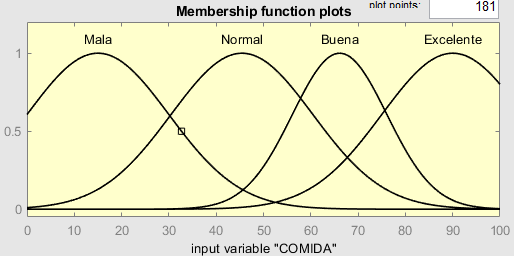
\includegraphics[width=0.8\textwidth]{IMG/G15.png}
		\end{figure}
		\newpage
		\item Baja ($\mu = 5.5$, $\sigma = 3$), Normal ($\mu = 12$, $\sigma = 3$) y Alta ($\mu = 12$, $\sigma = 2.5$).
		\begin{figure}[h]
			\centering
			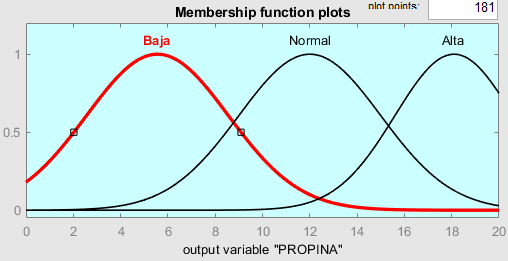
\includegraphics[width=0.8\textwidth]{IMG/G16.png}
		\end{figure}
	\end{enumerate}
	
	Se mantuvo el método de desfuzzificación del centroide para todas las funciones.\\
	
	A continuación se muestra el resultado de la gráfica de superficie con las modificaciones a las funciones de membresía: \\
	
	
	\begin{figure}[h]
		\centering
		\begin{subfigure}{0.42\textwidth} % Reducido de 0.45
			\centering
			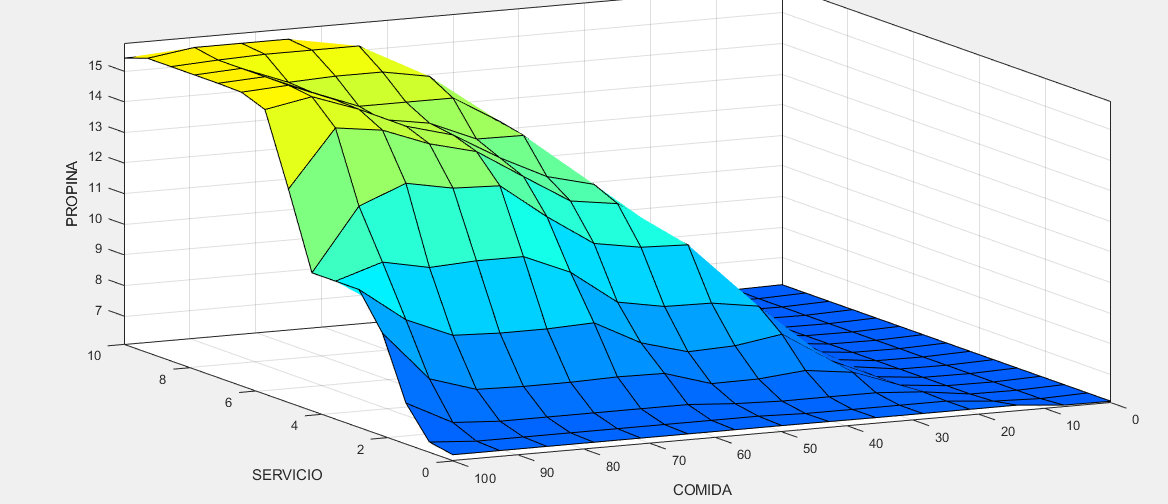
\includegraphics[width=1.3\textwidth]{IMG/G11.png}
			\label{fig:G11}
		\end{subfigure}
		\hfill
		\begin{subfigure}{0.42\textwidth} % Reducido de 0.45
			\centering
			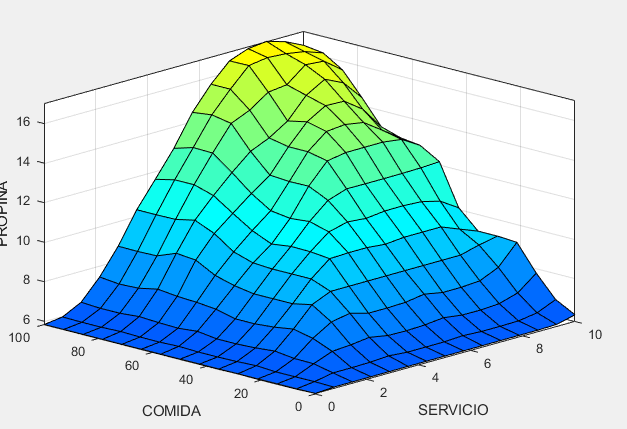
\includegraphics[width=1.2\textwidth]{IMG/G12.png}
			\label{fig:G12}
		\end{subfigure}
		\label{fig:comparacion}
	\end{figure}
	
	Se observa como el comportamiento de la gráfica logra verse más suave respecto al caso inicial, de forma que su máximo valor de propina que llega a dar es de 16.9\%.
	
	\newpage
	
	Complementariamente, se muestra la gráfica de las reglas, que bajo condiciones casi ideales, el máximo de propina que logra alcanzar es del 16.9\%.
	
	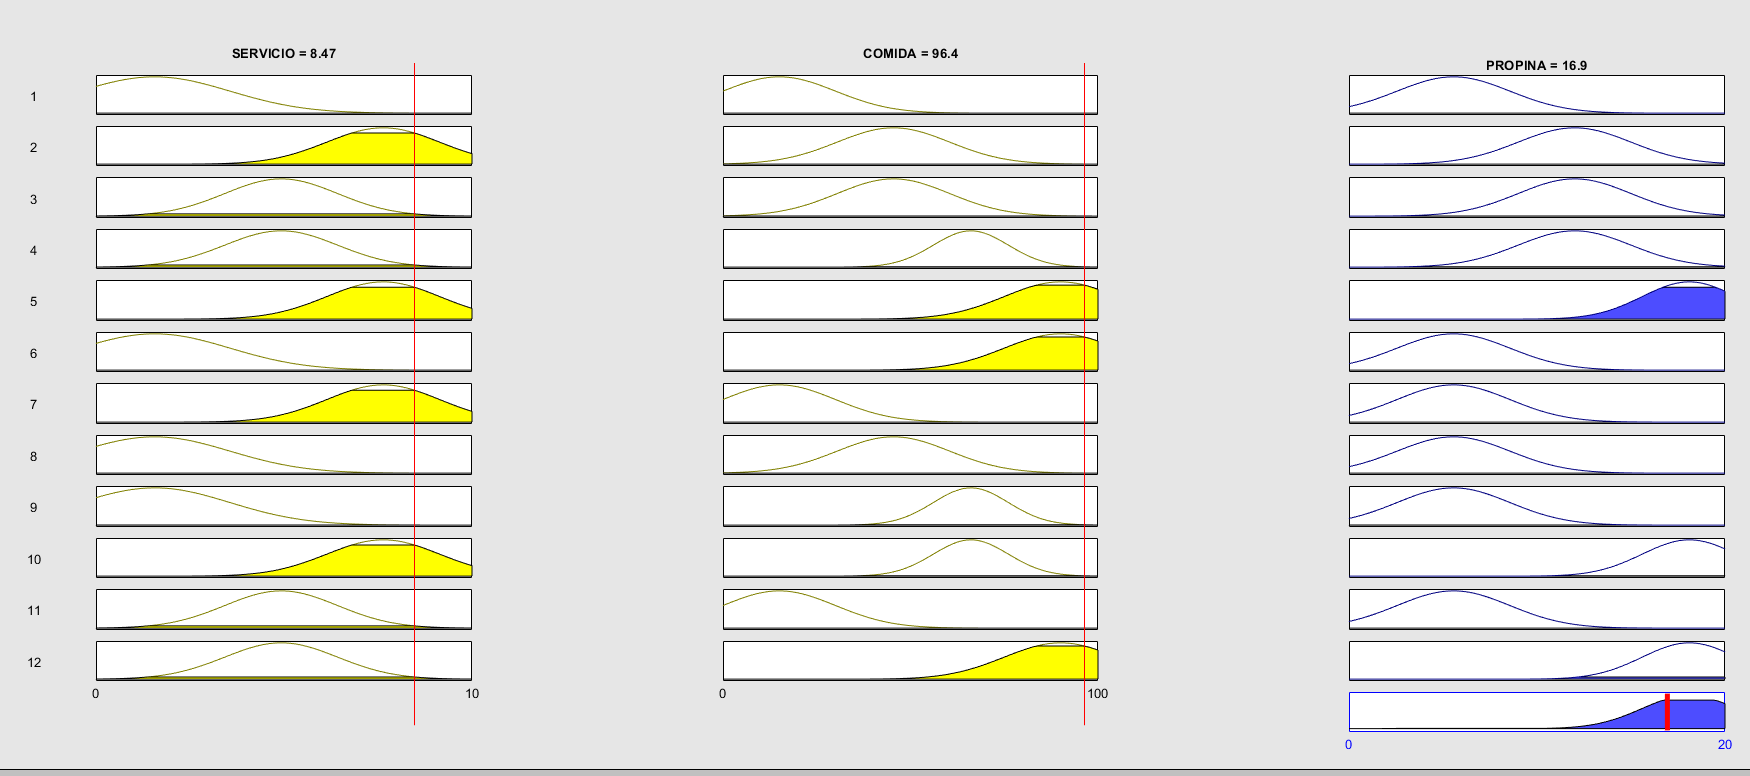
\includegraphics[width=1.1\textwidth]{IMG/G17.png}
	
	\subsection{Conclusiones}
	
	Tras realizar el moldeamiento del problema del mesero en su estado base y después de implementarlo con funciones gaussianas, se llega a la conclusión de que es crucial la selección adecuada de los rangos y las funciones de membresía, que la selección de las reglas no es algo trivial, deben ser incorporadas unicamente aquellas que tengan sentido dentro del contexto del problema.
	
	Se presenta la comparativa entre el caso inicial y el mejor caso obtenido con el modelamiento de funciones de membresía Gaussianas.
	
	\begin{figure}[h]
		\centering
		\begin{subfigure}{0.42\textwidth} % Reducido de 0.45
			\centering
			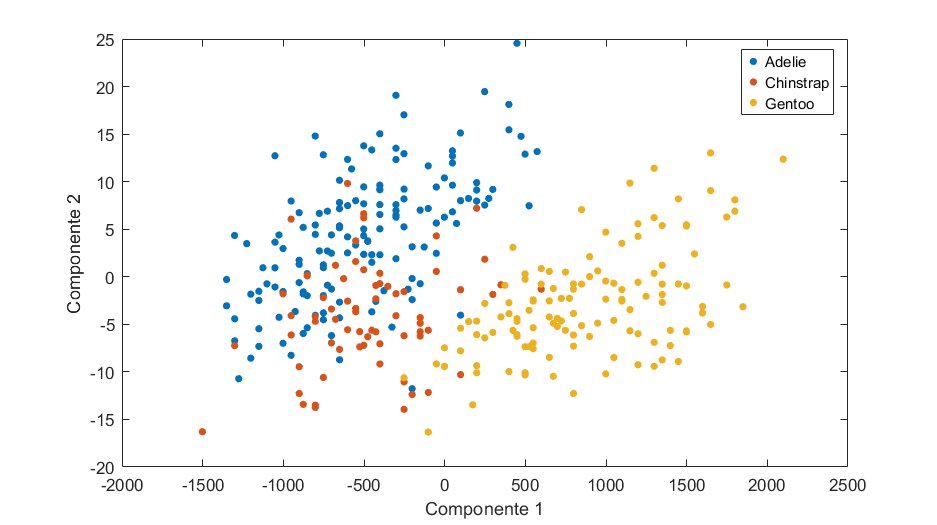
\includegraphics[width=1.3\textwidth]{IMG/G4.png}
			\label{fig:G111}
		\end{subfigure}
		\hfill
		\begin{subfigure}{0.42\textwidth} % Reducido de 0.45
			\centering
			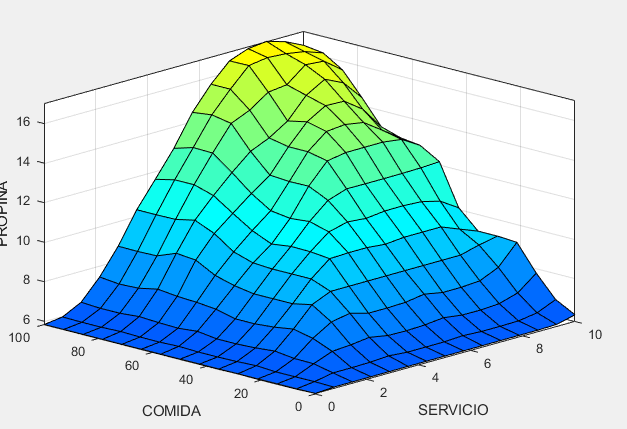
\includegraphics[width=1.2\textwidth]{IMG/G12.png}
			\label{fig:G112}
		\end{subfigure}
		\label{fig:comparacion2}
	\end{figure}
	
	
	
	\newpage
	
	
	% Sección para el problema 2
	\section{Problema 2: Problema del comfort y el clima.}
	
	\subsection{Explicación del Problema}
	
	Se tiene el problema más especifico de determinar el confort que tiene una persona dadas las variables  de temperatura y humedad en el ambiente.
	
	
	\subsection{Variables y sus codificaciones}
	
	
	A continuación se listan los valores de las variables lingüísticas que se propusieron para TEMPERATURA, HUMEDAD y COMFORT como sigue:
	
	
	\begin{enumerate}
		\item Temperatura: Frio (0 a 7.5), Fresco (2.5 a 15), Idóneo (12 a 20) y Calurosa (16 a 30).
		\begin{figure}[h]
			\centering
			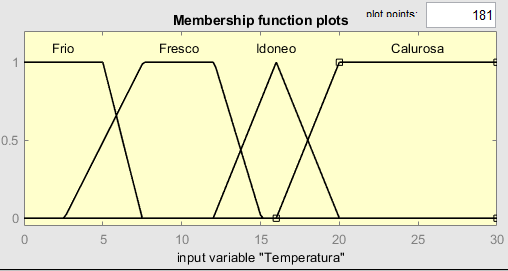
\includegraphics[width=0.8\textwidth]{IMG/G18.png}
		\end{figure}
		
		\item Humedad: Baja (0 a 25), Media (12 a 70) y Alta (55 a 100).
		\begin{figure}[h]
			\centering
			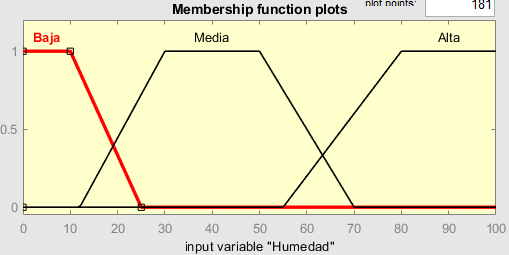
\includegraphics[width=0.8\textwidth]{IMG/G19.png}
		\end{figure}
		\newpage
		\item Confort: Mala (0 a 3), Incomoda (1.5 a 8) y Cómoda (6 a 10).
		\begin{figure}[h]
			\centering
			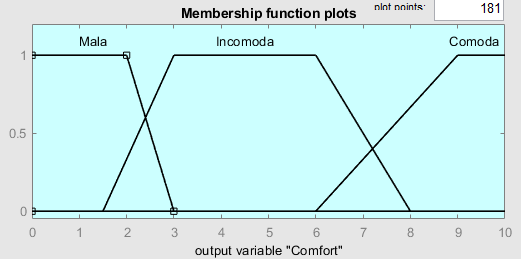
\includegraphics[width=0.8\textwidth]{IMG/G20.png}
		\end{figure}
	\end{enumerate}
	
	Cabe mencionar que todas las funciones de membresía se están modelando haciendo uso de la función trapezoidal a excepción del caso muy particular de la variable de TEMPERATURA en la etiqueta de IDÓNEO, para ese único caso se hizo uso de una función de membresía triangular. El método de defuzzificación de centroide fue utilizado para todas las funciones de membresía. \\
	
	Posterior a la propuesta de los rangos de calificación para la humedad y la temperatura, así como la determinación del grado de confort que va de 0 a 10, se procede con el diseño de la base del conocimiento para que sea posible realizar las inferencias para el porcentaje de propina.
	
	\subsection{Reglas de inferencia.}
	
	A continuación se muestran las diez reglas que se construyeron para este problema:
	
	\begin{enumerate}
		\item R1: Si \textbf{TEMPERATURA} es \textbf{\textit{FRÍO}} y la \textbf{HUMEDAD} es \textbf{\textit{BAJA}}, el \textbf{CONFORT} es \textbf{\textit{INCÓMODA}}.
		\item R2: Si \textbf{TEMPERATURA} es \textbf{\textit{FRESCO}} y la \textbf{HUMEDAD} es \textbf{\textit{BAJA}}, el \textbf{CONFORT} es \textbf{\textit{CÓMODA}}.
		\item R3: Si \textbf{TEMPERATURA} es \textbf{\textit{IDÓNEO}} y la \textbf{HUMEDAD} es \textbf{\textit{BAJA}}, el \textbf{CONFORT} es \textbf{\textit{CÓMODA}}.
		\item R4: Si \textbf{TEMPERATURA} es \textbf{\textit{FRÍO}} y la \textbf{HUMEDAD} es \textbf{\textit{MEDIA}}, el \textbf{CONFORT} es \textbf{\textit{CÓMODA}}.
		\item R5: Si \textbf{TEMPERATURA} es \textbf{\textit{IDÓNEO}} y la \textbf{HUMEDAD} es \textbf{\textit{MEDIA}}, el \textbf{CONFORT} es \textbf{\textit{MALA}}.
		\item R6: Si \textbf{TEMPERATURA} es \textbf{\textit{FRÍO}} y la \textbf{HUMEDAD} es \textbf{\textit{BAJA}}, el \textbf{CONFORT} es \textbf{\textit{INCÓMODA}}.
		\item R7: Si \textbf{TEMPERATURA} es \textbf{\textit{IDÓNEO}} y la \textbf{HUMEDAD} es \textbf{\textit{ALTA}}, el \textbf{CONFORT} es \textbf{\textit{INCÓMODA}}.
		\item R8: Si \textbf{TEMPERATURA} es \textbf{\textit{CALUROSA}} y la \textbf{HUMEDAD} es \textbf{\textit{BAJA}}, el \textbf{CONFORT} es \textbf{\textit{MALA}}.
		\item R9: Si \textbf{TEMPERATURA} es \textbf{\textit{CALUROSA}} y la \textbf{HUMEDAD} es \textbf{\textit{MEDIA}}, el \textbf{CONFORT} es \textbf{\textit{INCÓMODA}}.
		\item R10: Si \textbf{TEMPERATURA} es \textbf{\textit{CALUROSA}} y la \textbf{HUMEDAD} es \textbf{\textit{ALTA}}, el \textbf{CONFORT} es \textbf{\textit{MALA}}.
	\end{enumerate}
	
	\subsection{Gráficos}
	
	La gráfica de superficie resultante de todo lo descrito previamente, es la siguiente:
	
	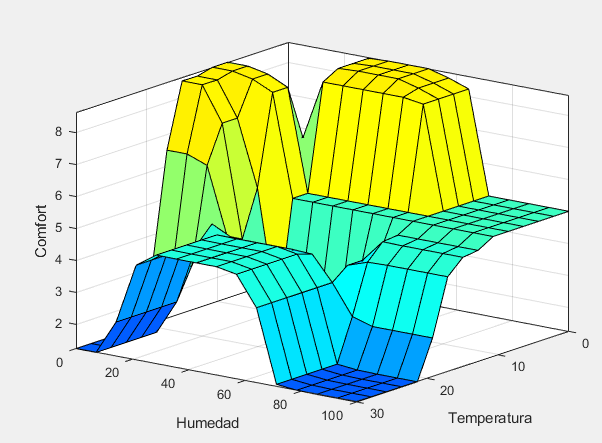
\includegraphics[width=0.8\textwidth]{IMG/G21.png}
	
	La superficie que se forma tiene una forma muy particular, puesto que dado las especificaciones del problema, se forma una región muy particular en donde la "comodidad" es alta, mientras que la maximización de alguna de las variables de entrada, puede derivar en el descenso repentino del indicador de comodidad.
	
	\newpage
	
	Complementariamente, se presenta la gráfica asociada a las reglas de inferencia. Se observa como es que lo máximo del indice de confort que se logra es apenas un valor de 5 en condiciones "optimas" de temperatura y humedad.\\
	
	
	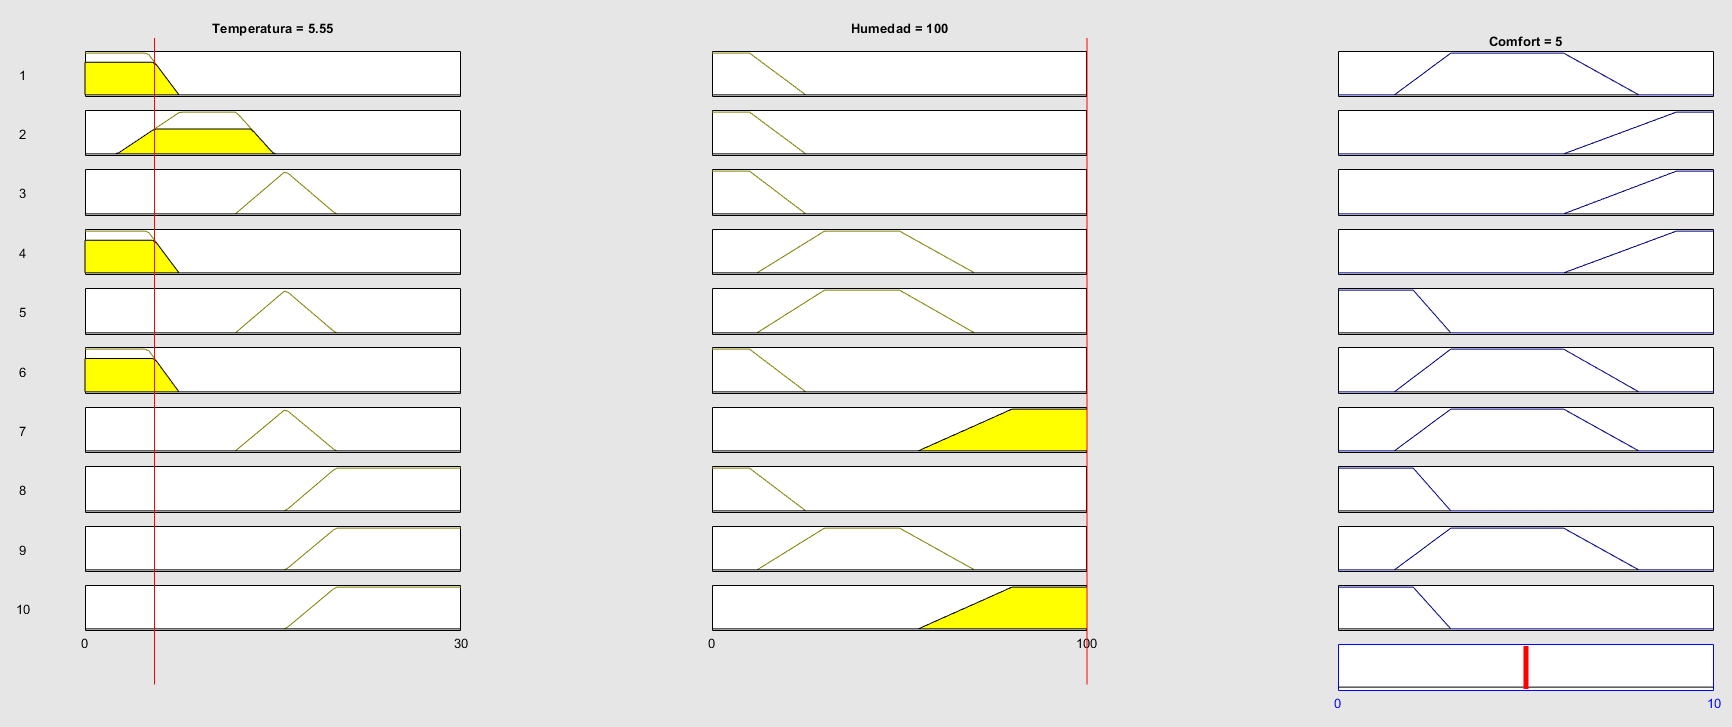
\includegraphics[width=1.1\textwidth]{IMG/G22.png}
	
	
	
	
	\newpage
	
	\subsection{Propuestas de mejora}
	
	\subsubsection{Propuesta 1: Base con 12 originales y aplicar funciones de membresía singleton}
	
	Como primer intento de mejorar la gráfica de superficie, se propone el uso de funciones de membresía singleton sobre las salidas de comfort:
	
	Se aplicaron los cambios de funciones de membresía para la variable COMFORT como se especifica a continuación
	
	\begin{enumerate}
		\item Mala (2), Incomoda (4) y Comoda (7).
		\begin{figure}[h]
			\centering
			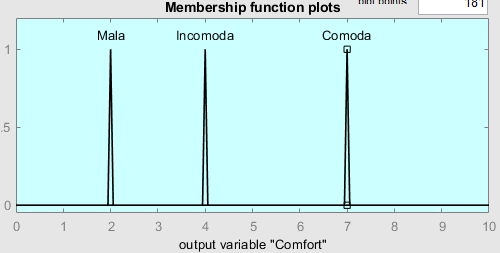
\includegraphics[width=0.8\textwidth]{IMG/G23.png}
		\end{figure}
	\end{enumerate}
	
	
	\newpage 
	
	La gráfica de superficie asociada a este cambio se muestra a continuación. \\
	
	
	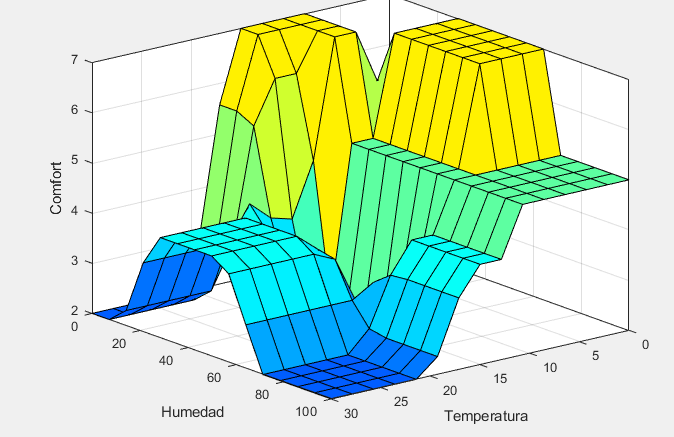
\includegraphics[width=0.8\textwidth]{IMG/G24.png} \\
	
	Se observa como el cambio de las salidas por funciones singleton produce una gráfica de superficie muy similar a la inicial, con la diferencia de que dicha gráfica no supera el indice de confort de 7. \\
	
	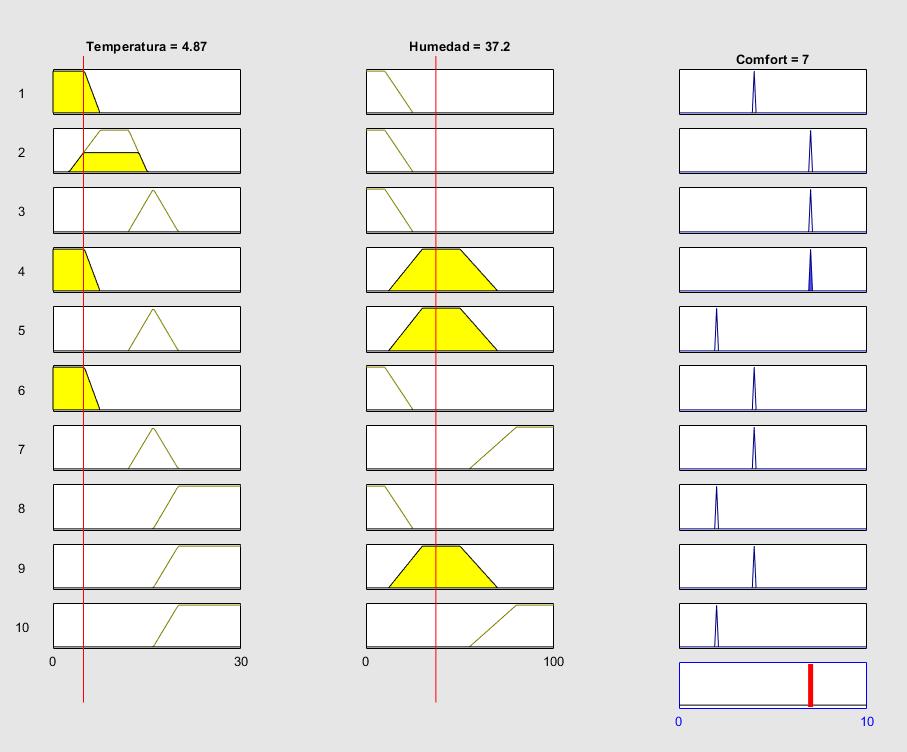
\includegraphics[width=1\textwidth]{IMG/G25.png}
	
	La gráfica de reglas muestra como pese a los valores tan puntuales del confort, la combinación de las reglas y de las variables de entrada logran abarcar los rangos para activar dichas funciones. \\
	
	\newpage
	
	\subsubsection{Propuesta 2: Base con las 10 reglas originales y aplicar funciones de membresía GAUSSIANAS}
	
	Con la finalidad de lograr suavizar la gráfica de superficie, se propone implementar cambios en los rangos de los valores de cada una de las variables lingüísticas y modificar sus funciones de membresía con gaussianas sin tocar las reglas ya construidas previamente.
	
	A continuación se listan los valores de las variables lingüísticas que se propusieron para TEMPERATURA, HUMEDAD y COMFORT como sigue:
	
	
	\begin{enumerate}
		\item Temperatura: Frio ($\mu = 0$, $\sigma = 3$), Fresco ($\mu = 11$, $\sigma = 3$), Idóneo ($\mu = 18$, $\sigma = 2.5$) y Calurosa ($\mu = 18$, $\sigma = 2.5$).
		\begin{figure}[h]
			\centering
			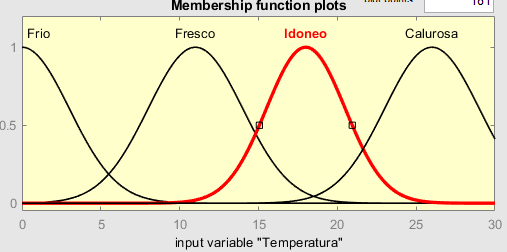
\includegraphics[width=0.8\textwidth]{IMG/G26.png}
		\end{figure}
		
		\item Humedad: Baja ($\mu = 20$, $\sigma = 10$), Media ($\mu = 40$, $\sigma = 15$) y Alta ($\mu = 80$, $\sigma = 15$).
		\begin{figure}[h]
			\centering
			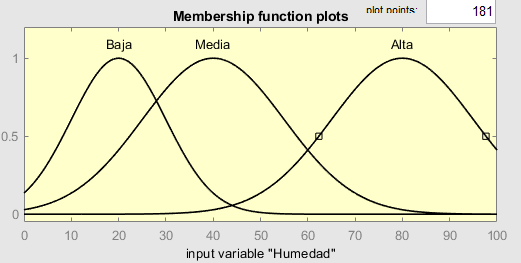
\includegraphics[width=0.8\textwidth]{IMG/G27.png}
		\end{figure}
		\newpage
		\item Confort: Malo ($\mu = 2$, $\sigma = 1$), Incomodo ($\mu = 4$, $\sigma = 1.5$) y Alta ($\mu = 9$, $\sigma = 2$).
		\begin{figure}[h]
			\centering
			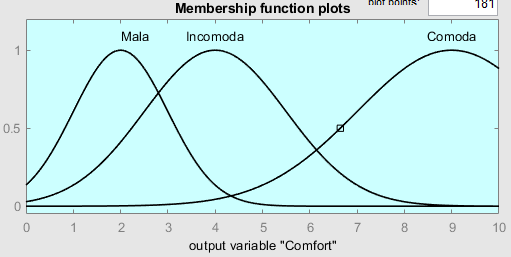
\includegraphics[width=0.8\textwidth]{IMG/G28.png}
		\end{figure}
	\end{enumerate}
	
	Se mantuvo el método de desfuzzificación del centroide para todas las funciones.\\
	
	A continuación se muestra el resultado de la gráfica de superficie con las modificaciones a las funciones de membresía: \\
	
	
	\begin{figure}[h]
		\centering
		\begin{subfigure}{0.42\textwidth} % Reducido de 0.45
			\centering
			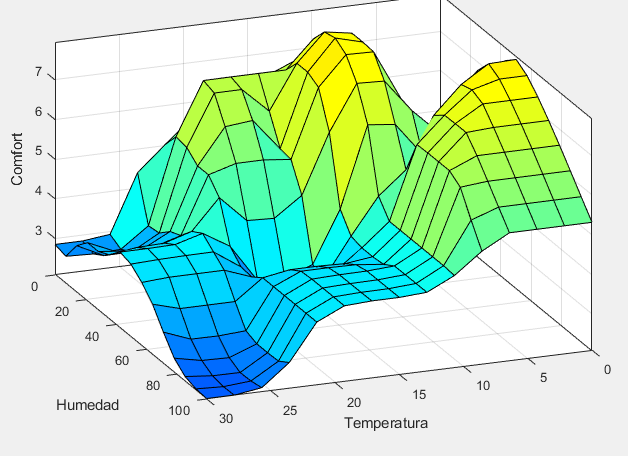
\includegraphics[width=1.3\textwidth]{IMG/G29.png}
			\label{fig:G21}
		\end{subfigure}
		\hfill
		\begin{subfigure}{0.42\textwidth} % Reducido de 0.45
			\centering
			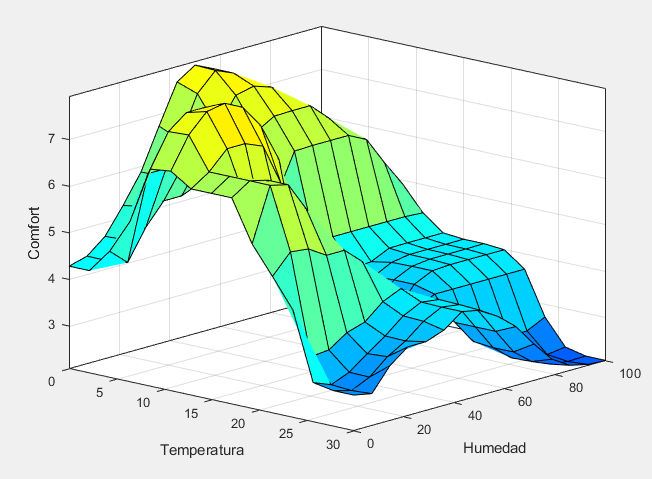
\includegraphics[width=1.2\textwidth]{IMG/G30.png}
			\label{fig:G22}
		\end{subfigure}
		\label{fig:comparacion3}
	\end{figure}
	
	Se observa como se logra suavizar de manera considerable respecto a la gráfica inicial que se veía más aplanada y con cambios abruptos muy marcados.
	
	\newpage
	
	Complementariamente, se muestra la gráfica de las reglas, que bajo condiciones casi ideales, el máximo indice de comodidad que logra alcanzar es de 7.95.
	
	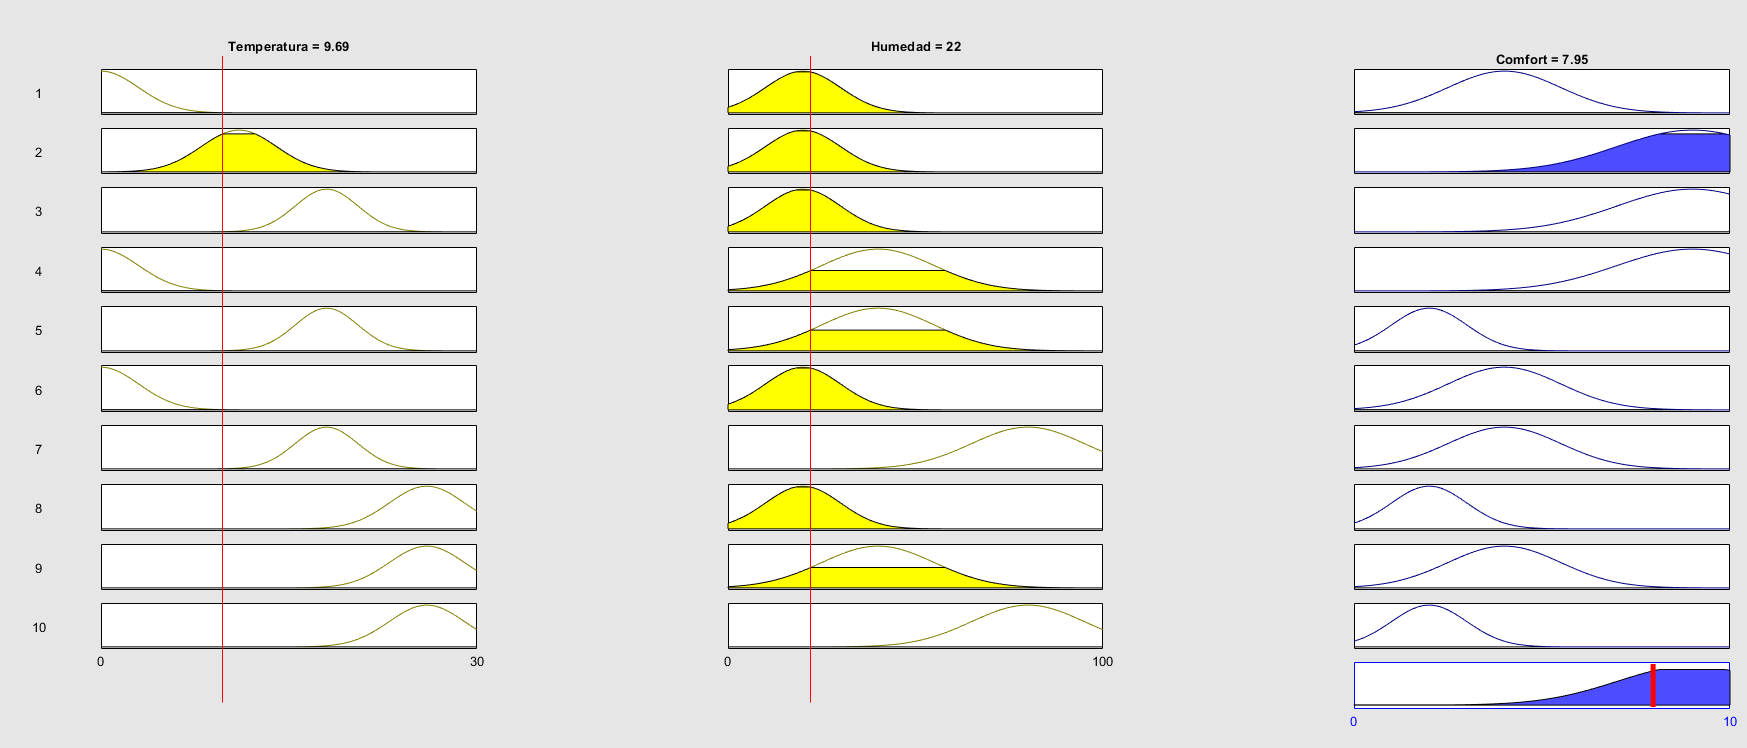
\includegraphics[width=1.1\textwidth]{IMG/G31.png}
	
	\subsection{Conclusiones}
	
	Tras realizar el ejercicio de modelar el problema de la humedad, la temperatura y el confort, se llega a la conclusión de que las funciones de membresía juegan un papel crucial en el suavizamiento de la gráfica de superficie, sin embargo, también es crucial el manejo adecuado de las reglas. Se sospecha que para este caso en particular, un arreglo de más fino de las reglas de la mano de un experto en el tema, lograrían que el gráfico presentara una forma aun más suave.
	
	Se presenta la comparativa entre el caso inicial y el mejor caso obtenido con el modelamiento de funciones de membresía Gaussianas.
	
	\begin{figure}[h]
		\centering
		\begin{subfigure}{0.42\textwidth} % Reducido de 0.45
			\centering
			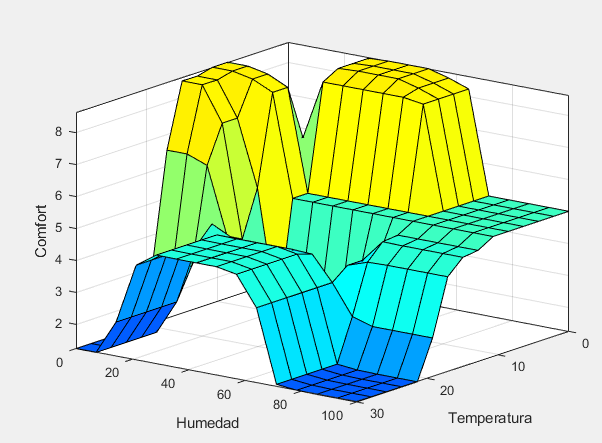
\includegraphics[width=1.3\textwidth]{IMG/G21.png}
			\label{fig:G211}
		\end{subfigure}
		\hfill
		\begin{subfigure}{0.42\textwidth} % Reducido de 0.45
			\centering
			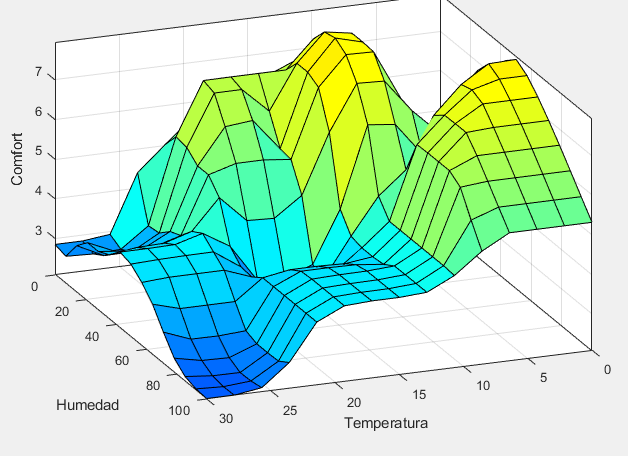
\includegraphics[width=1.2\textwidth]{IMG/G29.png}
			\label{fig:G212}
		\end{subfigure}
		\label{fig:comparacion4}
	\end{figure}
	
	
	
	\newpage
	
	
	
	
	
	
	
	
	
\end{document}

